\usepgfplotslibrary{fillbetween}

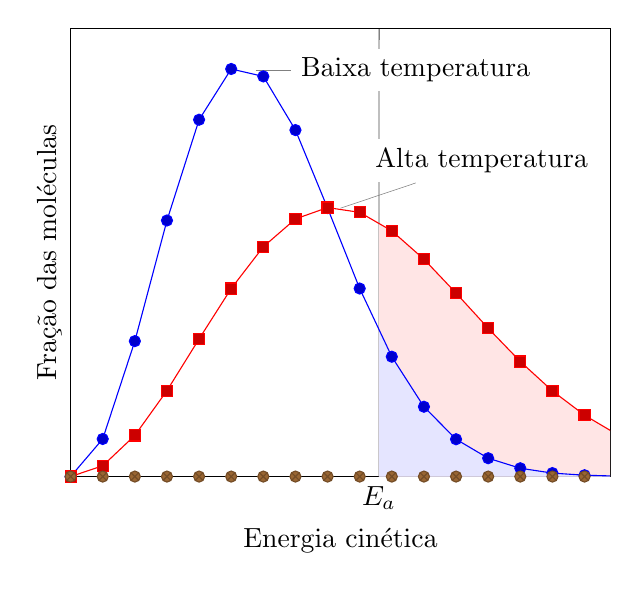
\begin{tikzpicture}
    \def\R{1000*8.314} % Constante de Boltzmann
    \begin{axis}
        [
            domain = 0:5000,
            xlabel = {Energia cinética},
            ylabel = {Fração das moléculas},
            xtick={2000}, 
            xticklabels = {$E_\text{a}$},
            grid = major,
            ytick = \empty,
            ymin=0,
            xmin=0, xmax = 3500,
        ]

    \node[coordinate, pin={[fill=white] right:{Baixa temperatura}}] 
        at (axis cs:1200,7.35e-4)   {};

    \node[coordinate, pin={[fill=white] above right:{Alta temperatura}}] 
        at (axis cs:1750,4.85e-4)   {};

    \pgfplotsinvokeforeach { 300, 700 }
        {
            \addplot+ [name path = #1]
                {
                    sqrt(2/pi)*(4/(\R*#1))^(3/2)*x^2*exp(-4/(\R*#1)*x^2/2)
                };
        }

    \addplot+[draw=none,name path=xaxis] {0};

    \addplot+[red!10] fill between 
        [of=700 and xaxis,soft clip={domain=2000:3500}];

    \addplot+[blue!10] fill between 
        [of=300 and xaxis,soft clip={domain=2000:3500}];
    
    \end{axis}
\end{tikzpicture}